\section{Terminarz realizacji poszczególnych podcelów}
    Lista podcelów z dokładnością do jednego tygodnia oraz wykres gantta (wykr. \ref{fig: gantt}):
\begin{itemize}
    \item 
        20.03.2023: Studia literatury 
    \item 
        27.03.2023: Projektowanie interfejsu graficznego
    \item 
        3.04.2023 : Projektowanie architektury systemu, projektowanie makiety i układu elektronicznego czujników
        \item PIERWSZY KAMIEŃ MILOWY: Ukończenie etapu projektowania
    \item 
        10.04.2023: Budowa makiety i układu elektronicznego czujników
    \item 
        17.04.2023: Testowanie działania układu elektronicznego czujników
    \item 
        24.04.2023: Implementacja głównych elementów GUI
    \item 
        1.05.2023: Implementacja głównych elementów GUI
    \item 
        8.05.2023: Testowanie głównych elementów GUI
    \item 
        15.05.2023: Implementacja komponentów logicznych aplikacji
    \item 
        22.05.2023: Testowanie komponentów logicznych aplikacji
    \item 
        29.05.2023: Implementacja pozostałych elementów GUI
    \item 
        5.06.2023: Testowanie pozostałych elementów GUI
    \item 
        12.06.2023: Integracja wszystkich komponentów, testowanie aplikacji
    \item 
        19.06.2023: Tworzenie raportu końcowego
    \item DRUGI KAMIEŃ MILOWY:  Złożenie raportu końcowego i prezentacja rezultatów
\end{itemize}

\begin{figure}
    \centering
    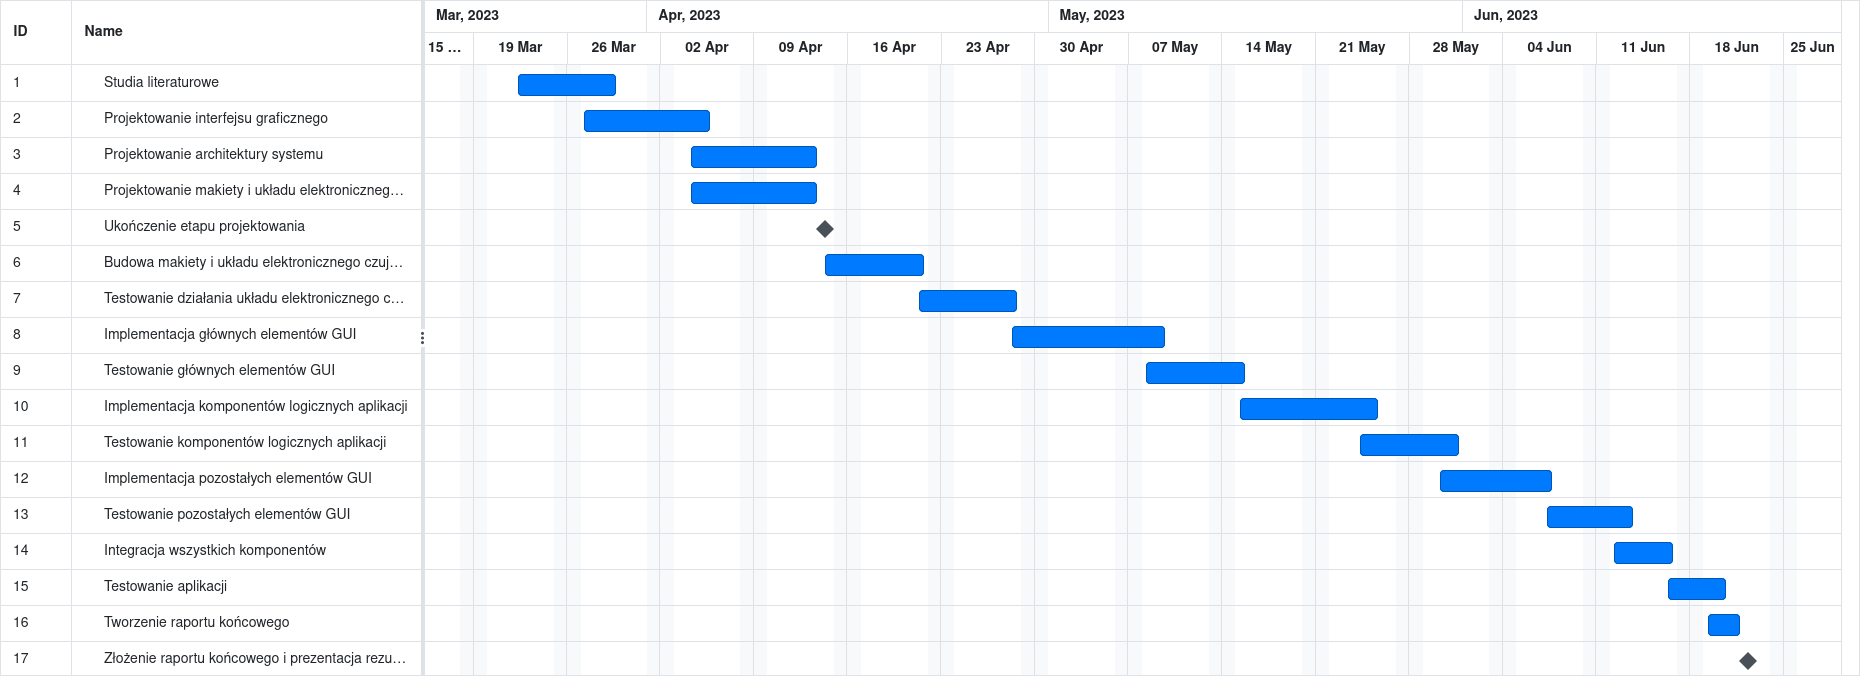
\includegraphics[width = \textheight, angle = 270]{obrazy/wsd_gantt.png}
    \caption{Wykres gantta}
    \label{fig: gantt}
\end{figure}
